\section{Introduction}




Large language models (LLMs) have become the foundation of modern AI agents in applications such as coding, web search, and medicine. As agent execution increasingly relies on frequent LLM invocations, inference efficiency has become a critical factor in both system throughput and user experience. Consequently, extensive research~\cite{zhou2024survey,li2024large} has explored various techniques to achieve extreme optimization on LLM inference, encompassing algorithm optimization~\cite{chen2026dflash,cheng2026dspark}, system enhancements~\cite{dao2022flashattention,hong2024flashdecoding++}, and hardware advancements~\cite{moon2024latency,prabhakar2024sambanova}.


% In the pursuit of artificial general intelligence, generative large language models (LLMs) have demonstrated tremendous potential and successfully enabled the development of various downstream applications, the most representative of which are agents in diverse scenarios (\textit{e.g.}, medicine~\cite{ferber2026towards}, coding~\cite{cc,codex}, and web search~\cite{xi2025survey}). Despite the rapid development of agentic applications, LLM inference remains the dominant computational component of agent execution, severely impacting the user experience. Consequently, extensive research~\cite{zhou2024survey,li2024large} has explored various techniques to achieve extreme optimization on LLM inference, encompassing algorithm optimization~\cite{chen2026dflash,cheng2026dspark,xu2025specee}, system enhancements~\cite{dao2022flashattention,hong2024flashdecoding++,dai2025flashdecoding++}, and hardware advancements~\cite{moon2024latency,prabhakar2024sambanova}.


Speculative decoding has emerged as a mainstream inference acceleration technique, which has been widely adopted by prominent LLMs (\textit{e.g.}, DeepSeek-V4~\cite{xu2026deepseek}) and deployed in real-world serving systems(\textit{e.g.}, SGLang~\cite{zheng2024sglang} and vLLM~\cite{kwon2023efficient}). A lightweight draft model first generates multiple candidate tokens, which are then verified by the target model in a single forward pass. By accepting multiple tokens at once, speculative decoding can substantially improve inference efficiency without compromising accuracy.


% Speculative decoding has emerged as a mainstream inference acceleration technique, which has been widely adopted by prominent LLMs (\textit{e.g.}, DeepSeek-V4~\cite{xu2026deepseek} and GLM-5.2~\cite{zeng2026glm}) and deployed in real-world serving systems(\textit{e.g.}, SGLang~\cite{zheng2024sglang} and vLLM~\cite{kwon2023efficient}). Its basic principle is to use a lightweight draft model to generate speculative candidate tokens, which are subsequently verified by the target model before the accepted tokens are committed to the output sequence. By accepting multiple tokens through a single forward pass of the target model, the acceptance length can directly translate into inference speedup without compromising accuracy, effectively alleviating the low throughput and poor GPU utilization caused by token-by-token generation over the full context in autoregressive decoding. 

However, agentic workloads differ significantly from conventional conversational inference. As illustrated in Figure~\ref{fig:agent}(a), agent execution typically involves long inputs, short outputs, frequent multi-turn interactions, and continuously growing contexts. Under such workloads, we observe two major limitations of existing speculative decoding methods. \textbf{(1) From the perspective of algorithmic performance},  Figure~\ref{fig:agent}(b) shows that the methods that achieve high acceptance lengths on conventional benchmarks can drop to only \(1\sim2\) accepted tokens on agentic workloads, corresponding to a degradation of more than \(80\%\). Lightweight draft models increasingly struggle to independently model the long historical context required to match the predictive distribution of the target model. \textbf{(2) From the perspective of system efficiency}, maintaining the draft model's historical states introduces non-negligible system overhead. Existing speculative drafters must continuously update their KV cache with newly accepted tokens and maintain historical states for subsequent generation and prefix reuse. Under frequent multi-turn agent execution, these operations can account for \(10\%\sim20\%\) of end-to-end inference latency.


% These two limitations share a common source: the draft model is required to independently encode and maintain an increasingly long history, even though the target model has already processed the same context. This observation motivates a different design principle: rather than reconstructing the full history inside the draft model, the drafter should directly reuse contextual representations produced by the target model and focus its own capacity on local speculative prediction.
These two limitations share a common source: the draft model is required to independently encode and maintain an increasingly long history, though the target model has processed the same context. More importantly, this growing history continuously increases the explicit context length and positional range faced by the lightweight drafter, making the prediction problem increasingly difficult. We therefore adopt a different design principle: \textbf{rather than reconstructing the full history inside the draft model, the drafter directly reuses contextual representations produced by the target model and performs only local speculative prediction around the current decoding position.} 

Based on this insight, we propose \we, a history-free speculative decoding framework for agentic AI. \we employs a history-free parallel backbone that directly consumes target hidden states and performs local prediction around the current decoding position without maintaining historical draft KV cache. A lightweight sequential head restores the missing intra-block causal dependency directly in the hidden space, avoiding expensive intermediate vocabulary projections. Finally, we introduce a two-stage training strategy that first bridges the structural mismatch using an isomorphic history-aware teacher and then directly aligns \we with the target model. 

We train \we for Qwen3-4B, Qwen3-8B models and evaluate it on both general-purpose, long-context and agentic workloads. \we achieves \(2\sim6\) acceptance length and improves over DSpark by up to \(70\%\), completely eliminating the draft model's historical KV-cache maintenance overhead.


\begin{figure}[!t]
    \centering
    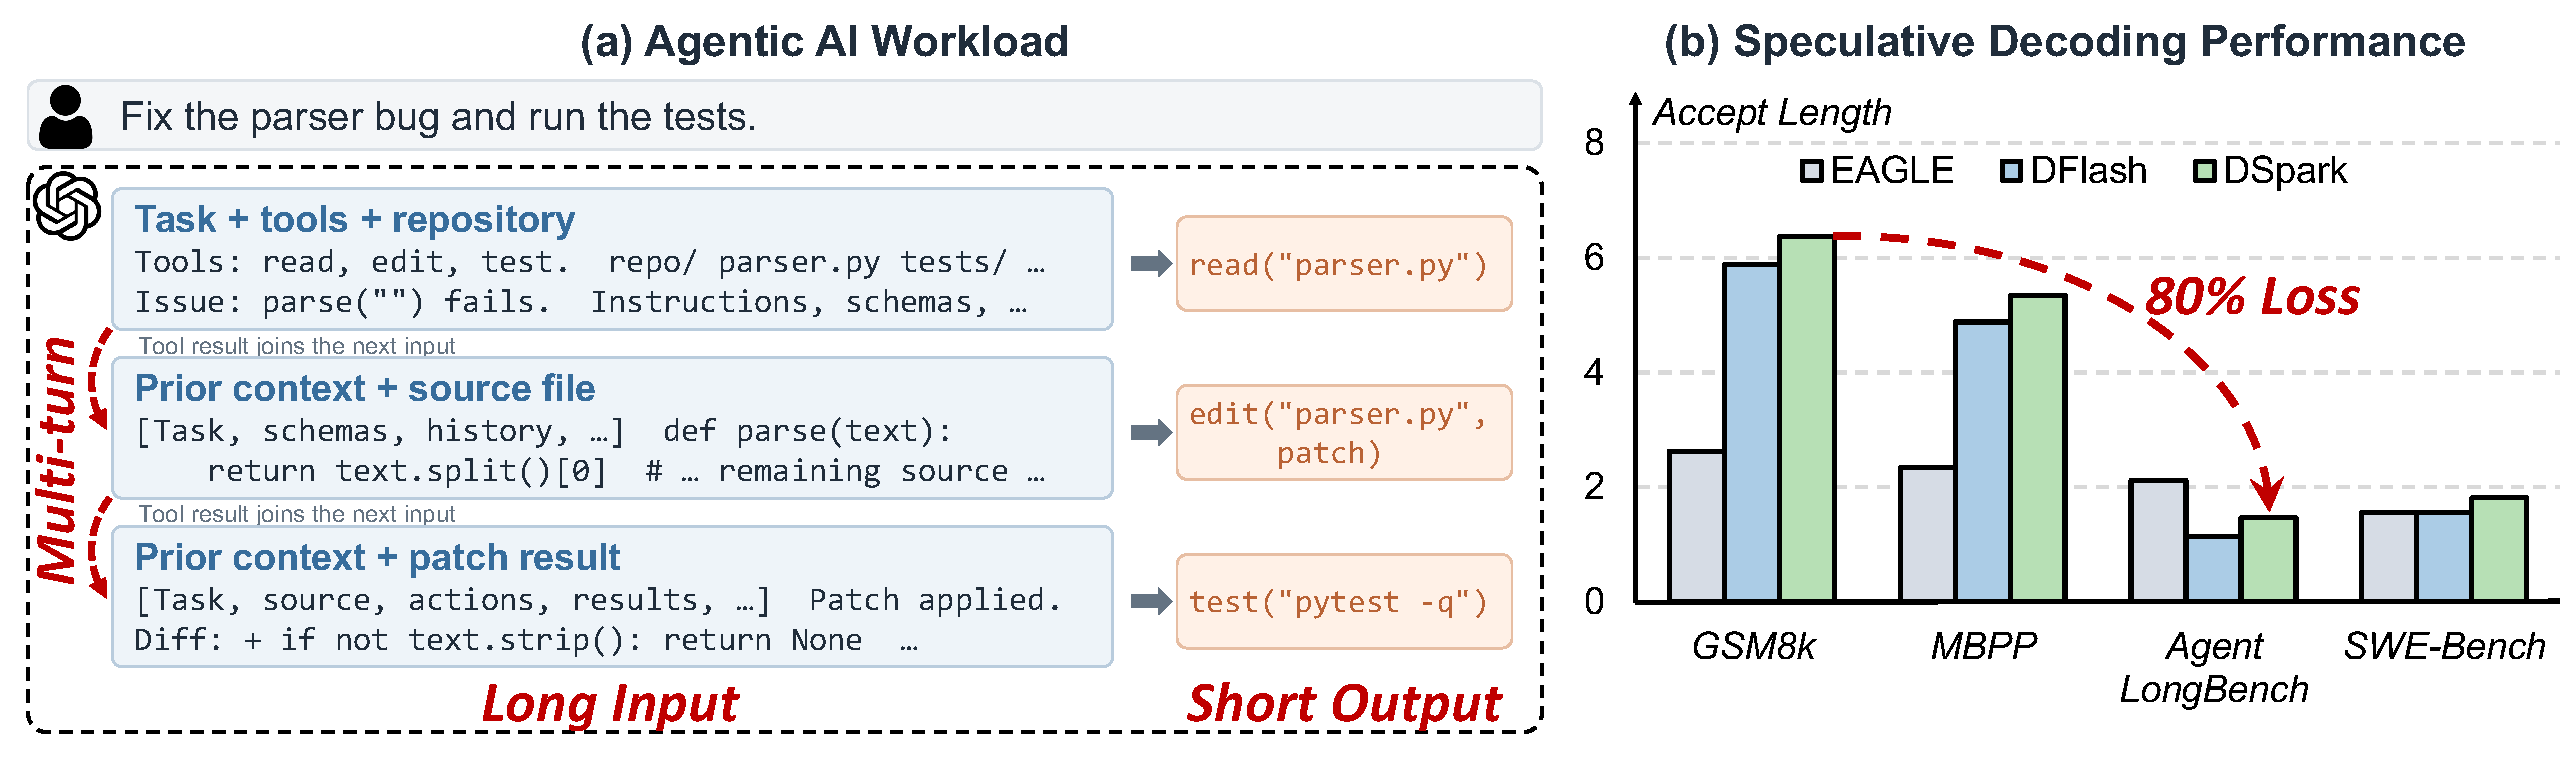
\includegraphics[width=0.98\textwidth]{fig/agent.pdf}
    \caption{(a) Agentic workloads characteristics. (b) Speculative decoding performance loss.}
    \vspace{-10pt}
    \label{fig:agent}
\end{figure}
% However, as agentic applications become increasingly mature, the computational workload characteristics handled by inference systems have fundamentally shifted. Unlike conventional requests in conversational AI, requests in agentic AI exhibit strong heterogeneity and runtime uncertainty in terms of context composition, sequence length, and execution paths due to the introduction of the harness~\cite{dsh}. This results in a unique workload profile: single-turn interactions typically feature long inputs but short outputs, while multi-turn interactions are characterized by high-frequency invocations and extended conversational depths. Under such workloads, we observe that existing state-of-the-art speculative decoding methods (\textit{e.g.}, EAGLE~\cite{li2024eagle}, DFlash~\cite{chen2026dflash}) encounter significant challenges in both algorithmic performance and system efficiency, even when deployed on mature LLM serving systems.

% \textbf{(1) From the perspective of algorithmic performance}, state-of-the-art speculative decoding methods can achieve substantial acceptance lengths on conventional workloads (\textit{e.g.}, DFlash achieves an acceptance length of nearly 6 on GSM8K~\cite{chen2026dflash}). However, under agentic workloads characterized by long inputs and short outputs, their performance degrades by over 80\%, with the acceptance length dropping to only $1\sim2$ tokens. This degradation substantially limits the acceleration potential of speculative decoding in agentic scenarios.

% \textbf{(2) From the perspective of system efficiency}, existing speculative decoding methods require the draft model to update its KV cache with the tokens accepted by the target model after verification to maintain consistency. Moreover, the draft model must synchronously maintain the complete historical KV cache alongside the target model to support prefix caching optimizations across similar requests. The high-frequency and multi-turn nature of agentic workloads makes these KV cache states particularly expensive to maintain and update. This overhead can account for $10\%\sim30\%$ in end-to-end inference latency.

% Our analysis reveals that these two problems share the same fundamental cause: the continuously growing historical context. On the one hand, a lightweight draft model with limited parameters fails to match the capability of the target model on the long-context understanding, leading to a degraded acceptance length. On the other hand, the inference system is persistently burdened with updating and maintaining the draft model's KV cache generated by this growing context, resulting in suboptimal system efficiency. To this end, we introduce \we, a speculative decoding framework tailored for agentic AI that jointly considers algorithmic performance and system efficiency from the outset.




% \textbf{(1) In the model design phase,} to ensure both algorithmic performance and system efficiency, \we adopts a lightweight semi-autoregressive architecture with a history-free design. Instead of maintaining the complete historical context cache, \we consists of a parallel backbone that performs prediction using only hidden states from the target model together with a local group of anchor tokens, and a lightweight serial head that explicitly models the sequential dependency among tokens within the speculative block. 

% \textbf{(2) In the model training phase,} to fully unlock the potential of this architecture, \we further introduces a tailored two-stage training strategy, the warm-up stage and stable stage, with different distillation targets and loss functions. During the warm-up stage, we first  train an isomorphic draft model equipped with historical context and use it as the distillation target for \we. \we is further trained to fit the output distribution using Kullback-Leibler (KL) divergence, with the goal of bringing the history-free model into a stable optimization region. Since the ultimate objective of the draft model is to align with the target model's output distribution, the stable stage shifts the distillation target directly to the target model. In this stage, \we is trained using a joint loss function of Cross-Entropy (CE) and Total Variation (TV) distance.

% We have trained the \we model for Qwen3-4B, Qwen3-8B, Qwen3.5-4B and evaluate them on NVIDIA H800 GPU. Extensive experiments demonstrate that \we achieves 2$\times \sim 6\times$ speedup on both general and agent-specific datasets, outperforming the state-of-the-art speculative decoding method, DSpark, by $20\% \sim 40\%$. Crucially, \we effectively enhances the acceptance length in agentic scenarios while entirely eliminating the system overhead associated with updating and maintaining the KV cache.


